\documentclass[UTF8,12pt]{article}
% \usepackage{indentfirst}   % 用于首行自动缩进的宏包
\usepackage{lipsum}   % 用于随机生成文本的宏包
\usepackage{subfigure}  
\usepackage{graphicx}   
\usepackage{float}   
\usepackage{amsmath}
\usepackage{xcolor} 
\usepackage{tikz} 
\usepackage{booktabs} 
\usepackage[style=gb7714-2015]{biblatex}
\usepackage[colorlinks,linkcolor=blue,anchorcolor=blue,citecolor=green]{hyperref} 
\usetikzlibrary{arrows,shapes,chains}
\linespread{1.5}
\bibliography{ref.bib}

% 题目
\title{xxx report}
% 作者
\author{...}
% 日期
\date{\today}

% 正文
\begin{document}
\maketitle

\begin{abstract}
	\lipsum[11]\cite{denton2014exploiting}
\end{abstract}

% 目录
\newpage
\tableofcontents
\newpage

% 第一部分
\section{xxx}

% 子标题
\subsection{xxx}
\lipsum[11]

% 图表
\begin{figure}[H]	\centering
	\subfigure[Harr feature]{
		\label{fig:a} 
		\includegraphics[width=2cm,height=2cm]{fig/1.JPG}}
	\vfill
	\subfigure[Integrogram]{
		\label{fig:subfig:b} 
		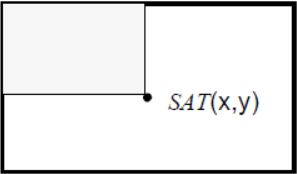
\includegraphics[width=2cm,height=1.8cm]{fig/2.JPG}}
	\qquad
	\subfigure[Calculate]{
		\label{fig:subfig:c} 
		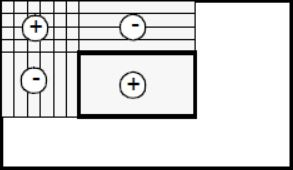
\includegraphics[width=2cm,height=1.8cm]{fig/3.JPG}}
	\caption{Schematic Diagram}
	\label{fig1} 
\end{figure}

\begin{figure}[H]
	\includegraphics[width=0.95\textwidth]{{fig/1.JPG}}
	\caption{FIG1}
	\label{fig_1}
\end{figure}

% 公式
\begin{equation} \label{eq:softquant}
\tilde{z}_i = \sum_{j=1}^L \frac{\exp(-\sigma\|z_i-c_j\|)}{\sum_{l=1}^L \exp(-\sigma\|z_i-c_l\|)} c_j
\end{equation}

% 流程图
	\begin{figure}[H]   \centering
		\scriptsize
		\tikzstyle{format}=[rectangle,draw,thin,fill=white,align=center]
		\tikzstyle{point}=[coordinate,on grid,]
		\begin{tikzpicture}[node distance=20mm,
		auto,>=latex',thin,start chain=going right,every join/.style={norm},]
		\node[point] (n0){PA};
		\node[format,right of=n0,node distance=17mm,] (n1){RGB to\\AXI-Stream};
		\node[format,right of=n1,node distance=20mm,] (n2){Image\\Processing};
		\node[format,right of=n2,node distance=17mm,] (n3){VDMA};
		\node[format,right of=n3,node distance=15mm,] (n4){DDR3};
		\node[format,right of=n4,node distance=14mm,] (n5){DDR3};	
		\draw[->] (n0.east) to node {Input} (n1);
		\draw[->] (n1.east) -- (n2);
		\draw[->] (n2.east) -- (n3);
		\draw[<->] (n3.east) to node {} (n4);
		\draw[<->] (n4.east) to node {} (n5);
		\end{tikzpicture}
		\caption{Flow Diagram}
		\label{fig2} 
	\end{figure}

% 子标题
\subsection{xxx}
\lipsum[11]
The table is shown below:
\begin{table}[H]
	\centering
	\caption{Three Wire Table}
	\label{fig3}
	\begin{tabular}{cccc}
		\toprule
		&PC(ms) &arm(ms) &fpga(ms)\\
		\midrule
		Open &100 &176 &322\\
		Close &223 &967 &178\\
		\bottomrule	
	\end{tabular}
\end{table}

% reference
\newpage
\begingroup
    \linespread{1}
    \printbibliography[title={Reference}]
\endgroup

\end{document}
